\documentclass[presentation, aspectratio=169]{beamer}

\usepackage{polyglossia}
\usepackage{amsmath}
\usepackage{amsfonts}
\usepackage{graphicx}
\usepackage{hyperref}

\setdefaultlanguage{french}
\graphicspath{{images/}}

\usetheme[sectionpage=progressbar]{metropolis}
\metroset{subsectionpage=progressbar}
\setbeamersize{text margin left=1em, text margin right=1em}

\DeclareMathOperator*{\argmax}{arg\ max}
\DeclareMathOperator*{\argmin}{arg\ min}


\title{Journée Jeunes Chercheuses/Chercheurs de FARE}
\subtitle{Ateliers (?)}
\date{20 janvier 2025}
\author{Alban Goupil}
\institute{%
  \hfill
  
\includegraphics[height=12mm]{urca-logo}
  \qquad
  
\includegraphics[height=12mm]{logocrestic}}

\begin{document}
\maketitle


\section{Projet DASY}

\begin{frame}{Problématique}
  \begin{itemize}
  \item Surveillance à grande échelle de l'évolution des jaunisses
  \item Flavescence Dorée
    \begin{itemize}
    \item Propagation rapide
    \item Traitement = arrachage
    \end{itemize}
  \item Détection manuelle = coût / temps
  \end{itemize}

  \centering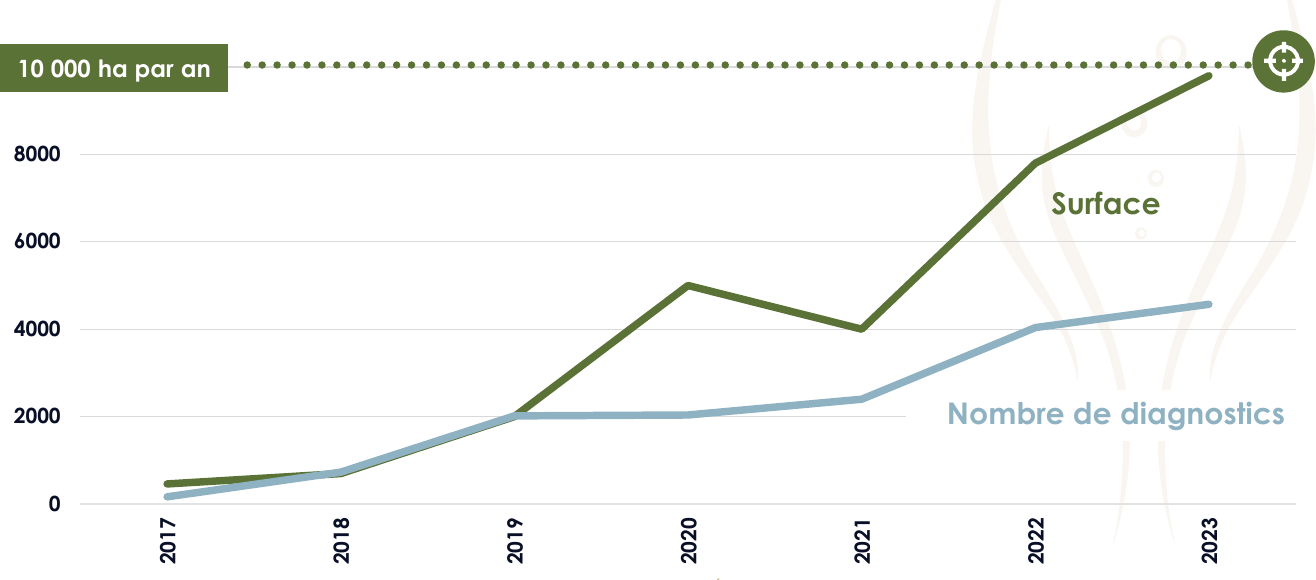
\includegraphics[width=10cm]{surveillance}
\end{frame}

\begin{frame}{DASY: Détection Automatisée des SYmptômes de jaunisse}
  \begin{columns}
    \column{.7\textwidth}
    \begin{block}{Objectifs}
      \begin{itemize}
      \item Extraction de bandes spectrales discriminantes
        \begin{itemize}
        \item Méthodes à développer
        \item Spécification de caméras multispectrales
        \item Acquisition à large échelle
        \end{itemize}
      \item Systèmes embarqués
        \begin{itemize}
        \item Transport sur nacelle / drone
        \item Mécatronique / robotique
        \end{itemize}
      \end{itemize}
    \end{block}

    \begin{block}{Consortium}
      \begin{itemize}
      \item Comité Champagne / CIVC
      \item SEGULA Technologies
      \item CReSTIC
      \end{itemize}
    \end{block}
    \column{.29\textwidth}
    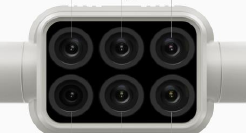
\includegraphics[width=.9\textwidth]{camera}
  \end{columns}
\end{frame}


\begin{frame}{Acquisition des spectres}
  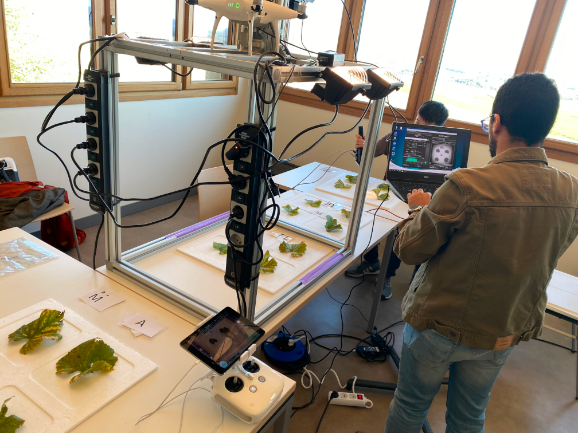
\includegraphics[height=4cm]{dispositif}
  \hfill
  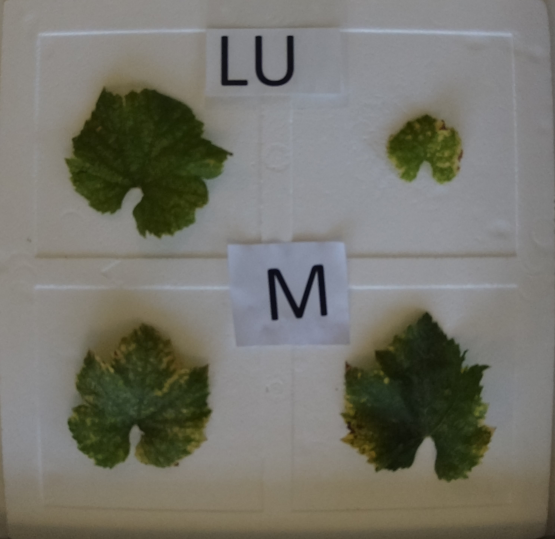
\includegraphics[height=4cm]{planches}
  \hfill
  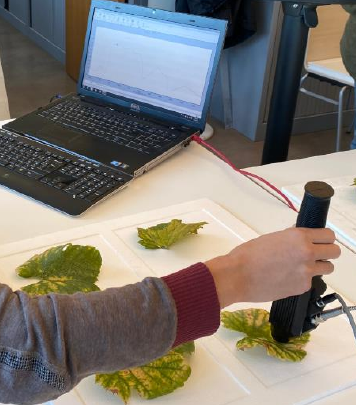
\includegraphics[height=4cm]{spectro}
  \begin{itemize}
  \item Spectres Vis + NIR allant de 350nm à 1350nm
  \item 2 spectres / feuilles
  \item Acquisitions de 2019 à 2024
  \item $\approx150$ ceps sur 5 zones avec 5 classes en 2022
  \end{itemize}
\end{frame}


\begin{frame}{Acquisition des images}
  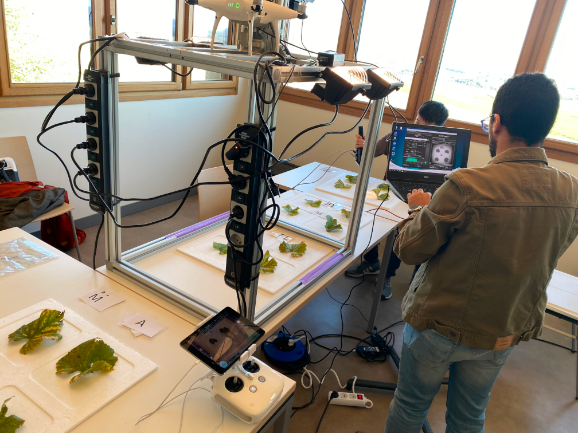
\includegraphics[height=35mm]{dispositif}
  \hfill
  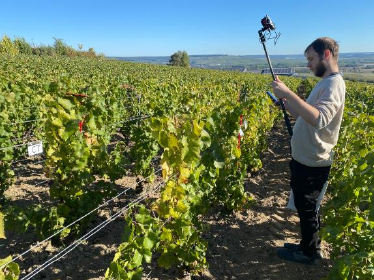
\includegraphics[height=35mm]{champs}  
  \hfill
  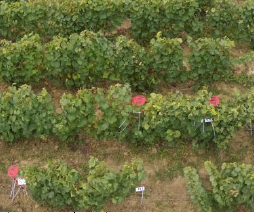
\includegraphics[height=35mm]{drone}
  \begin{itemize}
  \item Conditions contrôlées + hauteur nacelle + hauteur drone
  \item Données ci-dessous selon campagne de mesures 2022
  \item $\approx2400$ images de feuilles Vis-NIR + SWIR soit 31\ 000
    images
  \item $\approx150$ images de ceps Vis-NIR sur terrain $\times2$
    prises $\times3$ luminosités soit 3\ 600 images
  \item Acquisition drone artisanale Vis-NIR (5 bandes)
  \end{itemize}
\end{frame}


\section{Prise en main des données}

\begin{frame}{Étapes de la prise en main}
  \begin{itemize}
  \item Base de données: spectres de 2020
  \item Lecture des données en format CSV compressé
  \item Taille de la base \# observations / \# variables
  \item Visualisation / réduction de dimension
  \item Prétraitements
  \end{itemize}

  \begin{itemize}
  \item Site: \url{https://github.com/alban-goupil/jc-fare-2025}
  \item \href{https://github.com/alban-goupil/jc-fare-2025/blob/main/notebooks/1-prise-en-main.ipynb}{Notebook
      pour la prise en main}
  \end{itemize}
\end{frame}


\section{Premiers tests avec ML sur étagère}

\begin{frame}{Classifications}
  \begin{block}{Classificateurs utilisés}
    \begin{itemize}
    \item Support Vector Classifier (SVC)
    \item Random Forest (RF)
    \item Linear Discriminant Analysis (LDA)
    \end{itemize}
  \end{block}

  \href{https://github.com/alban-goupil/jc-fare-2025/blob/main/notebooks/2-classifieurs.ipynb}{Notebook
    sur la classification}
\end{frame}


\section{Qu'est-ce qu'un modèle ?}

\begin{frame}{Point de vue bayésien}
  \begin{itemize}
  \item L'équation de base
    \begin{equation*}
      \text{Modèle} = \text{Données} + \text{Préjugés}
    \end{equation*}
  \item Format mathématique = Bayes
    \begin{equation*}
      \underbrace{p(\text{Modèle}\mid \text{Données})}_{\text{a posteriori}}
        \propto \underbrace{p(\text{Données}\mid\text{Modèle})}_{\text{vraisemblance}}
        \times
        \underbrace{p(\text{Modèle})}_{\text{a priori}}
    \end{equation*}
  \item Modèle : architecture et paramètres
    \begin{itemize}
    \item Modèle linéaire : $y = ax+b$; architecture:
      équation droite, paramètres: $a$, $b$
    \item Réseaux de neurones : $y = f(x, w)$; architecture: réseaux
      de $n$ couches avec $m$ entrées, etc; paramètres: $w$
    \item GPT-3: $\text{token} = g(\text{token}, W)$; architecture:
      transformers et MLP; paramètres: $W = $175 milliards de nombres
    \end{itemize}
  \end{itemize}
\end{frame}

\begin{frame}{Modèle $\approx$ fonction indicatrice}
  \begin{block}{Approche probabiliste / énergétique}
    \begin{itemize}
    \item $p(x,y)$: probabilité de compatibilité entre $x$ et $y$
    \item $p(x,y)$ est une fonction à trouver en fonction du discours
    \item $p(x,y) \approx 1 \Longrightarrow \text{$x$ et $y$
        compatibles / accord}$
    \item $p(x,y) \approx 0 \Longrightarrow \text{$x$ et $y$
        incompatibles / désaccord}$
    \item Objectivisme (Fisher) / subjectivisme (Jaynes)
    \end{itemize}
  \end{block}

  \begin{block}{Exemples}
    \begin{itemize}
    \item
      $p(\raisebox{-.2\height}{
\includegraphics[width=5mm]{renard}},
      \text{renard}) = 90\%$
    \item
      $p(\raisebox{-.2\height}{
\includegraphics[width=5mm]{panda}},
      \text{renard}) = 20\%$
    \item $p(\text{"Il était une"}, \text{"fois"}) = 80\%$
    \item $p(\text{"Le plus grand groupe de rock est"}, \text{"Rolling
        Stones"}) = 0.1\%$
    \end{itemize}
  \end{block}
\end{frame}

\begin{frame}{Utilisation d'un modèle}
  \begin{center}\large
    $p(x, y) = p(x\mid y) \times p(y) = p(y\mid x) \times p(x)$
  \end{center}
  \begin{columns}[t]
    \column{.36\textwidth}
    \begin{block}{Modèle prédictif, régression}
      \begin{itemize}
      \item $\argmax_y p(y\mid x)$
      \item $\argmax_y
        p(y\mid\raisebox{-.2\height}{
\includegraphics[width=5mm]{panda}})
        = \text{panda}$
      \item
        $p(\text{renard}|\raisebox{-.2\height}{
\includegraphics[width=5mm]{renard}})=
        99\%$
      \item
        $p(\text{panda}|\raisebox{-.2\height}{
\includegraphics[width=5mm]{renard}})=
        1\%$
      \end{itemize}
    \end{block}
    \column{.64\textwidth}
    \begin{block}{Modèle génératif}
      \begin{itemize}
      \item $\argmax_x p(x\mid y)$
      \item $p(\text{"fois"}\mid \text{"Il était une"}) = 60\%$
      \item $p(\text{"Rolling Stones"}\mid \text{"Le meilleur groupe est"}) = 49\%$
      \item $p(\text{"Beattles"}\mid \text{"Le meilleur groupe est"})
        = 49\%$
      \end{itemize}
    \end{block}
  \end{columns}
\end{frame}

\begin{frame}{Apprentissage}
  \begin{align*}
    \text{Modèle}^\star
    &= \argmax_\text{Modèle}\quad p(\text{Modèle}\mid \text{Données})\\
    &= \argmax_\text{Modèle}\quad
      \underbrace{p(\text{Données}\mid\text{Modèle})}_{\text{Attachement
      aux données}}
    \times
    \underbrace{p(\text{Modèle})}_{\text{Architecture + régularisation}}
  \end{align*}
\end{frame}

\begin{frame}{Exemple}
  \begin{block}{Générateur de texte}
    \begin{itemize}
    \item Basé sur fréquences des $n$-grammes
    \item Apprentissage sur corpus de 3 livres français
    \item Architecture très simple
    \item Exemples digrammes $p(\text{es}) \approx 3.0\%$,
      $p(\text{le}) \approx 2.2\%$, $p(\text{qu}) \approx 1.1\%$,
      $p(\text{lz}) \approx 0\%$,
    \end{itemize}
  \end{block}

  \begin{block}{Liens externes}
    \begin{itemize}
    \item
      \href{https://github.com/alban-goupil/jc-fare-2025/blob/main/notebooks/3-modele-generateur.ipynb}{Notebook
        sur un générateur de texte}
    \item \href{https://www.inference.org.uk/dasher}{Dasher: un modèle
        prédictif pour l'écriture rapide}
    \end{itemize}
  \end{block}
\end{frame}


\section{Impact de la dimension}

\begin{frame}{Généralisation et régularité}
  \begin{columns}
    \column{.5\textwidth}
    \begin{block}{Problématique}
      \begin{itemize}
      \item Données d'entraînement
        \begin{itemize}
        \item[$\Longrightarrow$] toutes les données / entrées
        \end{itemize}
      \item Mesure de généralisation?
        \begin{itemize}
        \item[$\Longrightarrow$] données test
        \end{itemize}
      \end{itemize}
    \end{block}
    \begin{block}{Solution}
      \begin{itemize}
      \item Nécessité de régularité
      \item Échantillon représentatif
        \begin{itemize}
        \item[$\Longrightarrow$] recouvrement / pavage de l'espace des
          entrées possibles
        \end{itemize}
      \item Le hasard fait bien les choses
      \end{itemize}
    \end{block}
    \column{.49\textwidth}
    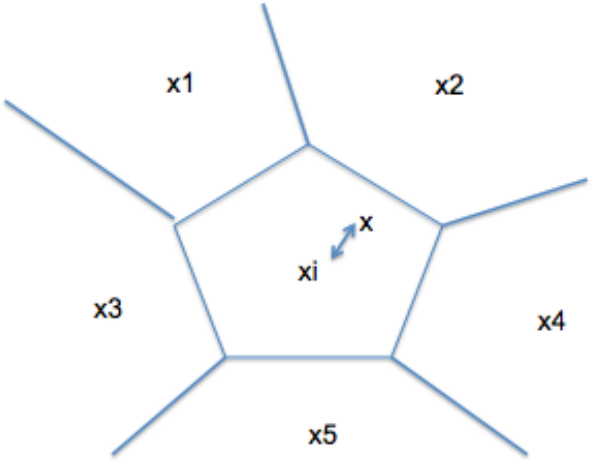
\includegraphics[width=\textwidth]{knn}
  \end{columns}
\end{frame}


\begin{frame}[squeeze]{Malédiction de la dimension}
  \begin{block}{Pavage}
    \begin{itemize}
    \item Un point ``couvre'' un rayon de $\epsilon=0.1$
    \item Il faut $\approx10$ points pour couvrir le segment de
      longueur 1
    \item Il faut $\approx100$ points pour couvrir le carré de côté 1
    \item Il faut $\approx1000$ points pour couvrir le cube de côté 1
    \item Il faut plus de $\epsilon^{-d}\left[\frac d{2\pi
          e}\right]^{d/2}$ points dans un hypercube de côté 1
    \item \alert{Réponse: concentration de la mesure}
    \end{itemize}
  \end{block}

  \begin{columns}
    \column{.8\textwidth}
    \begin{block}{Autres phénomènes de la dimension
        \href{https://github.com/alban-goupil/jc-fare-2025/blob/main/notebooks/4-dimension.ipynb}{(notebook
          illustratif)}}
      \begin{itemize}
      \item Tout l'espace est loin des données
        \begin{itemize}
        \item ``Dans l'(hyper)-espace personne ne vous entend crier.''
        \end{itemize}
      \item Toutes les directions sont orthogonales
      \item Durcissement des sphères / toute la masse est à l'équateur
      \end{itemize}
    \end{block}
    \column{.18\textwidth}
    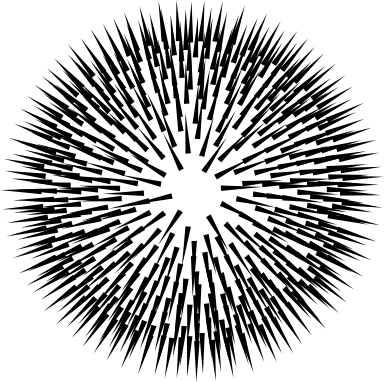
\includegraphics[width=\textwidth]{spiked-ball}
  \end{columns}
\end{frame}


\section{Impact du nombre d'observations}

\begin{frame}{Bayes pour expliquer l'impact}
  \begin{block}{Bayes cas dans le cas des données i.i.d}
    \begin{equation*}
      \log p(M\mid D) = \log p(M) + \sum_{i=1}^n \log p(D_i|M)
    \end{equation*}
    \begin{itemize}
    \item $M$: modèle, $D_i$: $i$-ème données sur $n$
    \item Si $n\approx 0$ alors l'\textit{a priori} est prédominant
    \item Si $n\to\infty$ alors l'\textit{a priori} devient
      négligeable
      \begin{itemize}
      \item \href{https://doi.org/10.1098/rsta.2018.0145}{Succi, Coveney, 2019, Big data: the end of the scientific method?}
      \end{itemize}
    \item
      \href{https://github.com/alban-goupil/jc-fare-2025/blob/main/notebooks/5-observations.ipynb}{Notebook
        illustratif}
    \end{itemize}
  \end{block}
\end{frame}


\begin{frame}{Dilemme Biais-Variance}
  \begin{columns}
    \column{.59\textwidth}
    \begin{equation*}
      R(f_I) \le \tilde R(\tilde f) \le R(f_I)
      + 2\max_{h\in\mathcal H}\lvert R(h) - R(\tilde h)\rvert
    \end{equation*}
    \begin{itemize}
    \item $R(.)$: Erreur de généralisation
    \item $\mathcal H$: ensemble des estimateurs possibles
    \item $f_I$: meilleur estimateur avec toutes les données possibles
      et inimaginables
    \item $\tilde f$: meilleur estimateur avec les données
    \end{itemize}
    \column{.4\textwidth}
    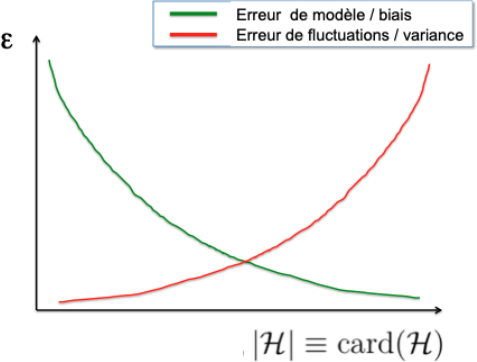
\includegraphics[width=\textwidth]{biais-variance}
  \end{columns}
\end{frame}


\begin{frame}{Sur-apprentissage et double descente}
  \centering
  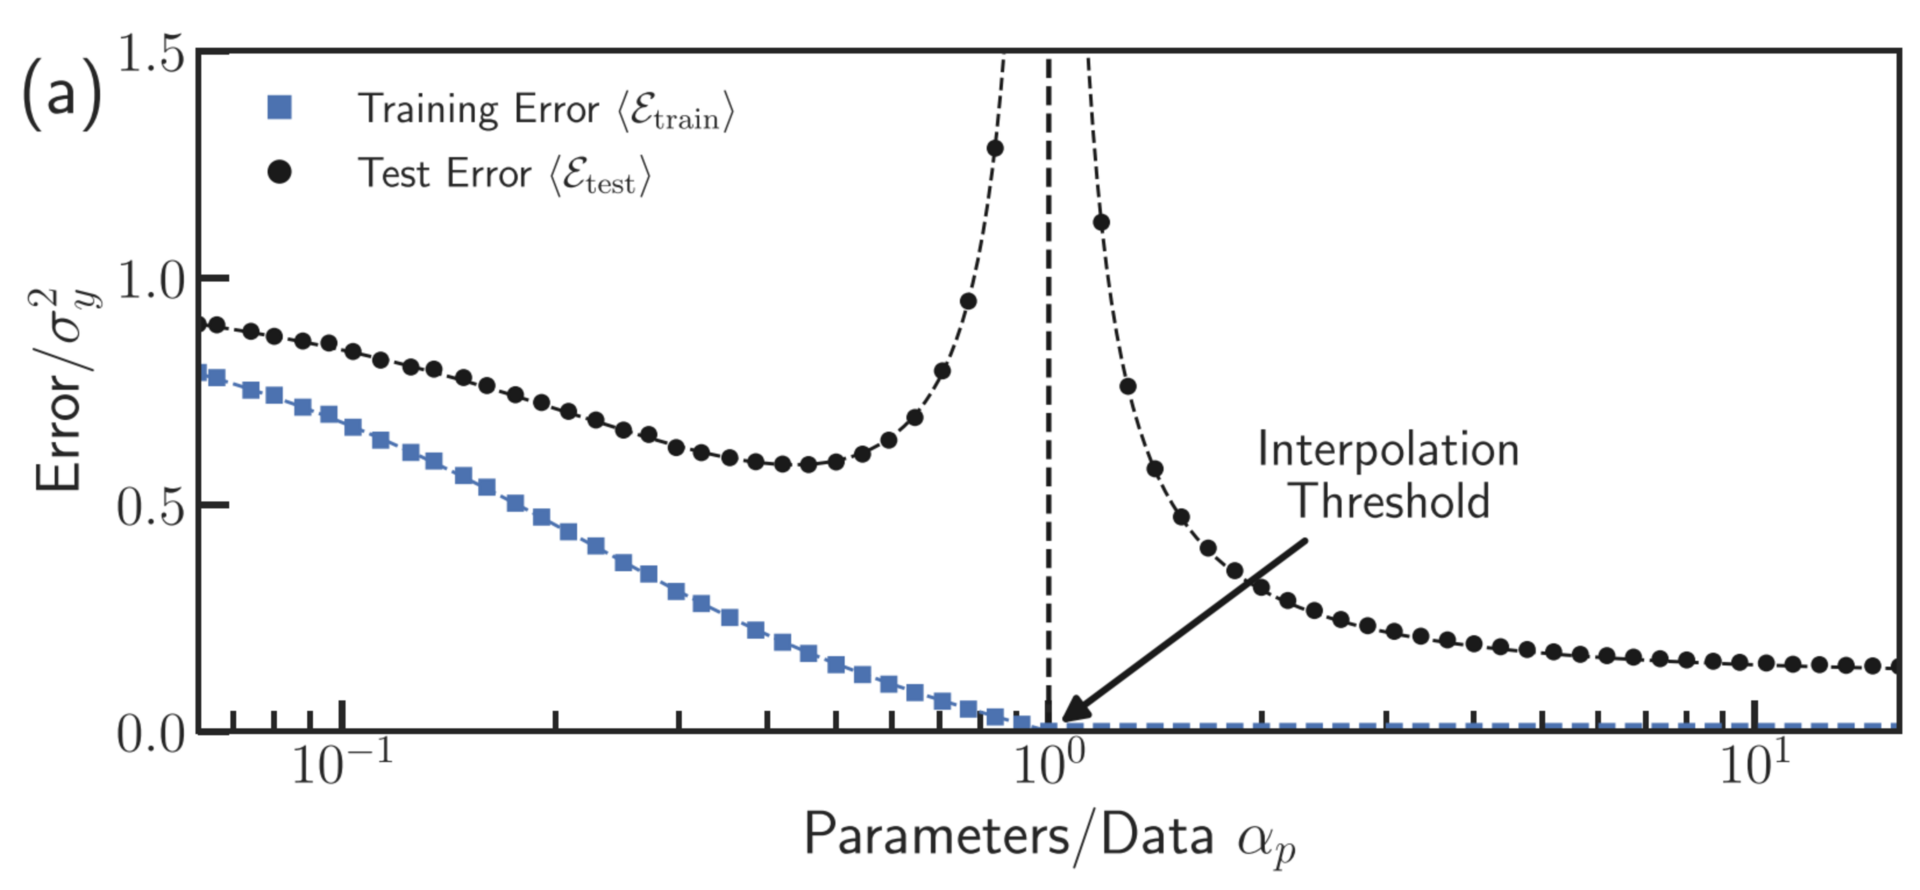
\includegraphics[width=.7\textwidth]{double-descente}
  \begin{alertblock}{Sur-apprentissage}
    \begin{columns}
      \column{.49\textwidth}
      \begin{itemize}
      \item \# paramètres $\gg$ \# données
      \item Mémorisation des données d'entraînement
      \end{itemize}
      \column{.49\textwidth}
      \begin{itemize}
      \item Généralisation remise en cause
      \item Nécessité de régularisation
      \end{itemize}
    \end{columns}
  \end{alertblock}
\end{frame}


\section{Sélection de variables}

\begin{frame}{Création d'un indice de jaunissité}
  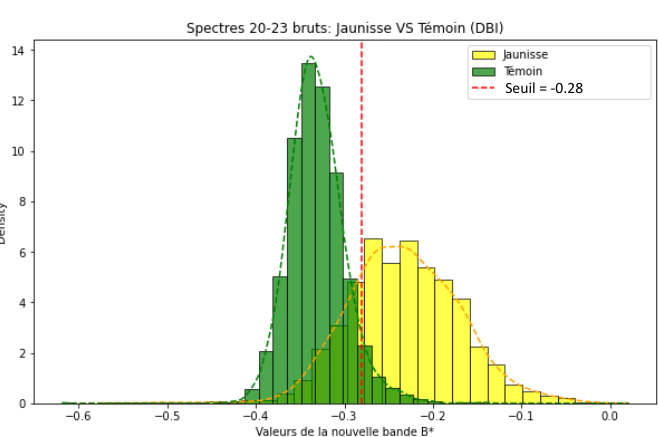
\includegraphics[height=5cm]{jaunisse-temoin-hist}
  \hfill
  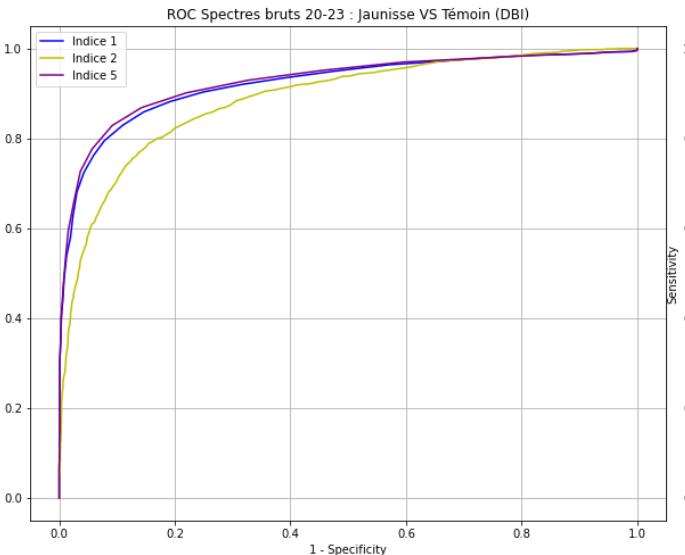
\includegraphics[height=5cm]{jaunisse-temoin-roc}
  \begin{columns}
    \column{.5\textwidth}
    \begin{itemize}
    \item Indice 1 = 3 bandes (2 Vis + 1 NIR)
    \item Indice 2 = 3 bandes (2 Vis + 1 NIR)
    \item Indice 5 = 4 bandes (2 Vis + 2 NIR)
    \end{itemize}
    \column{.49\textwidth}
    \centering
    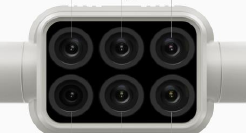
\includegraphics[height=2cm]{camera}
  \end{columns}
\end{frame}

\begin{frame}{Exemple de méthode de sélection}
  \begin{itemize}
  \item Utilisation du CorEx pour regrouper les variables
  \item Trouver les liaisons classes / bandes
  \item Mais bandes agnostiques aux années
  \end{itemize}
  \begin{center}
    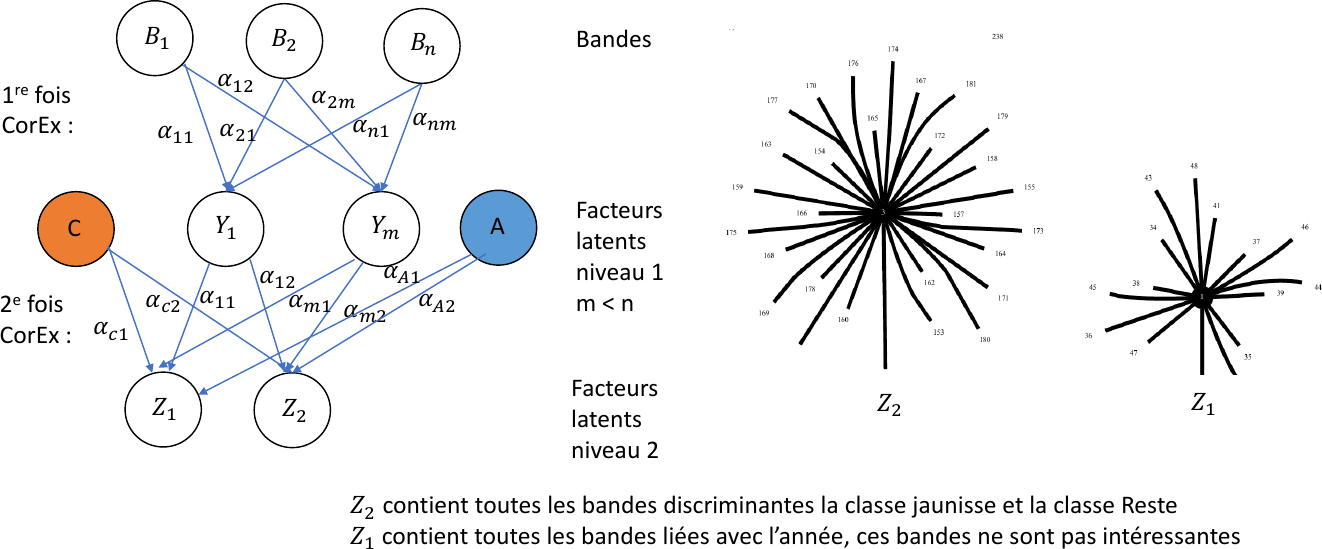
\includegraphics[width=.9\textwidth]{corex}
  \end{center}
\end{frame}


\section{Pour finir}

\begin{frame}{Conclusion}
  \begin{itemize}
  \item Outils de l'apprentissage automatique = puissants + simples
    à manipuler
  \item Véritables points critiques
    \begin{enumerate}
    \item Expertise des opérateurs / a priori / préjugé
    \item Qualité des données
    \item Critique des résultats
    \item Choix des modèles et de la méthode d'apprentissage
    \item Connaissances des limites des outils
    \end{enumerate}
  \item Aide d'expertes en science des données = points 4 et 5
    \begin{itemize}
    \item[$\Longrightarrow$] Bouclage entre experts du domaine et du ML
    \end{itemize}
  \end{itemize}
\end{frame}
\end{document}
